\clearpage
\section{Data sets and simulated samples}
\label{sec:datasets}

This section provides details about the simulated samples and data samples used in the analysis. Simulation is used both for he signal, as well as for SM processes.

\subsection{Standard Model simulated samples}
\label{sec:sm-mc}

Simulation of SM events is used for the BDT training, closure tests and to aid a general understanding. Simulated FullSim Drell-Yan (DY) samples are also used to estimate the Z$\rightarrow\tau\tau$ background and to derive a transfer factor for background between a Z$\rightarrow\tau\tau$-enriched CR and the SR.

Most SM processes including QCD, leptonic W decays, top-antitop quark decays and Drell-Yan processes were simulated using \MGvATNLO~\cite{Alwall_2011} and \PYTHIA 8~\cite{Sj_strand_2015}, while single-top and leptonic WW diboson processes were simulated using \POWHEG BOX~\cite{Oleari_2010}.
Several \CMSSW releases were used to process the SM Monte Carlo (MC) samples.
The 2016 samples were reconstructed mainly in 9\_4\_X (RunIISummer16MiniAODv3). The 2017 MC samples were reconstructed in a 9\_4\_X (RunIIFall17MiniAODv2) release while the 2018 were reconstructed in a 10\_2\_X release. These samples use full CMS detector simulation, which is performed using the {\GEANTfour} toolkit~\cite{AGOSTINELLI2003250}.


\subsection{Signal simulated samples}
\label{sec:signal-simulation}

Signal events corresponding to the 2016, 2017, and 2018 data taking periods are simulated with the \PYTHIA 8.205 event generator at LO with the CUETP8M1 tune, based on the \textsc{nnpdf2.3lo}~\cite{Ball:2013hta} parton distribution function (PDF). All production processes are generated simultaneously using the \textsc{PYTHIA} option for inclusive production (\texttt{susy:all = on}), which includes all possible processes and not only those indicated in Fig. \ref{fig:signal-feynman-diagrams}. The relative rates of each process is proportional to its corresponding LO cross section. The total cross section is subsequently re-weighted to match the cross section computed with NLO plus next-to-leading-log (NLL) precision in the limit of mass-degenerate higgsino $\PSGczDt$, $\PSGcpmDo$,  and $\PSGczDo$ with all the other 
sparticles assumed to be heavy and decoupled.

Generated events are subsequently processed with the CMS fast detector
simulation program FastSim~\cite{Abdullin:2011zz,Giammanco:2014bza},
which yields results that are generally consistent with those from {\GEANTfour}. For each model point,  $5\cdot 10^5$ events have been generated in the grid represented in Fig \ref{fig:signal-scan-grid}. To achieve higher statistical precision for the same computing requirements, only the subset of events passing a generator-level event filter consisting of the requirement $\HT>180 \GeV$ has been simulated using FastSim. $\HT$ is computed as the scalar sum of the $\pt$ of generator-level AK4 jets with $\pt>30$ GeV and $\eta<5.0$.

\begin{figure}[!htb]
\centering
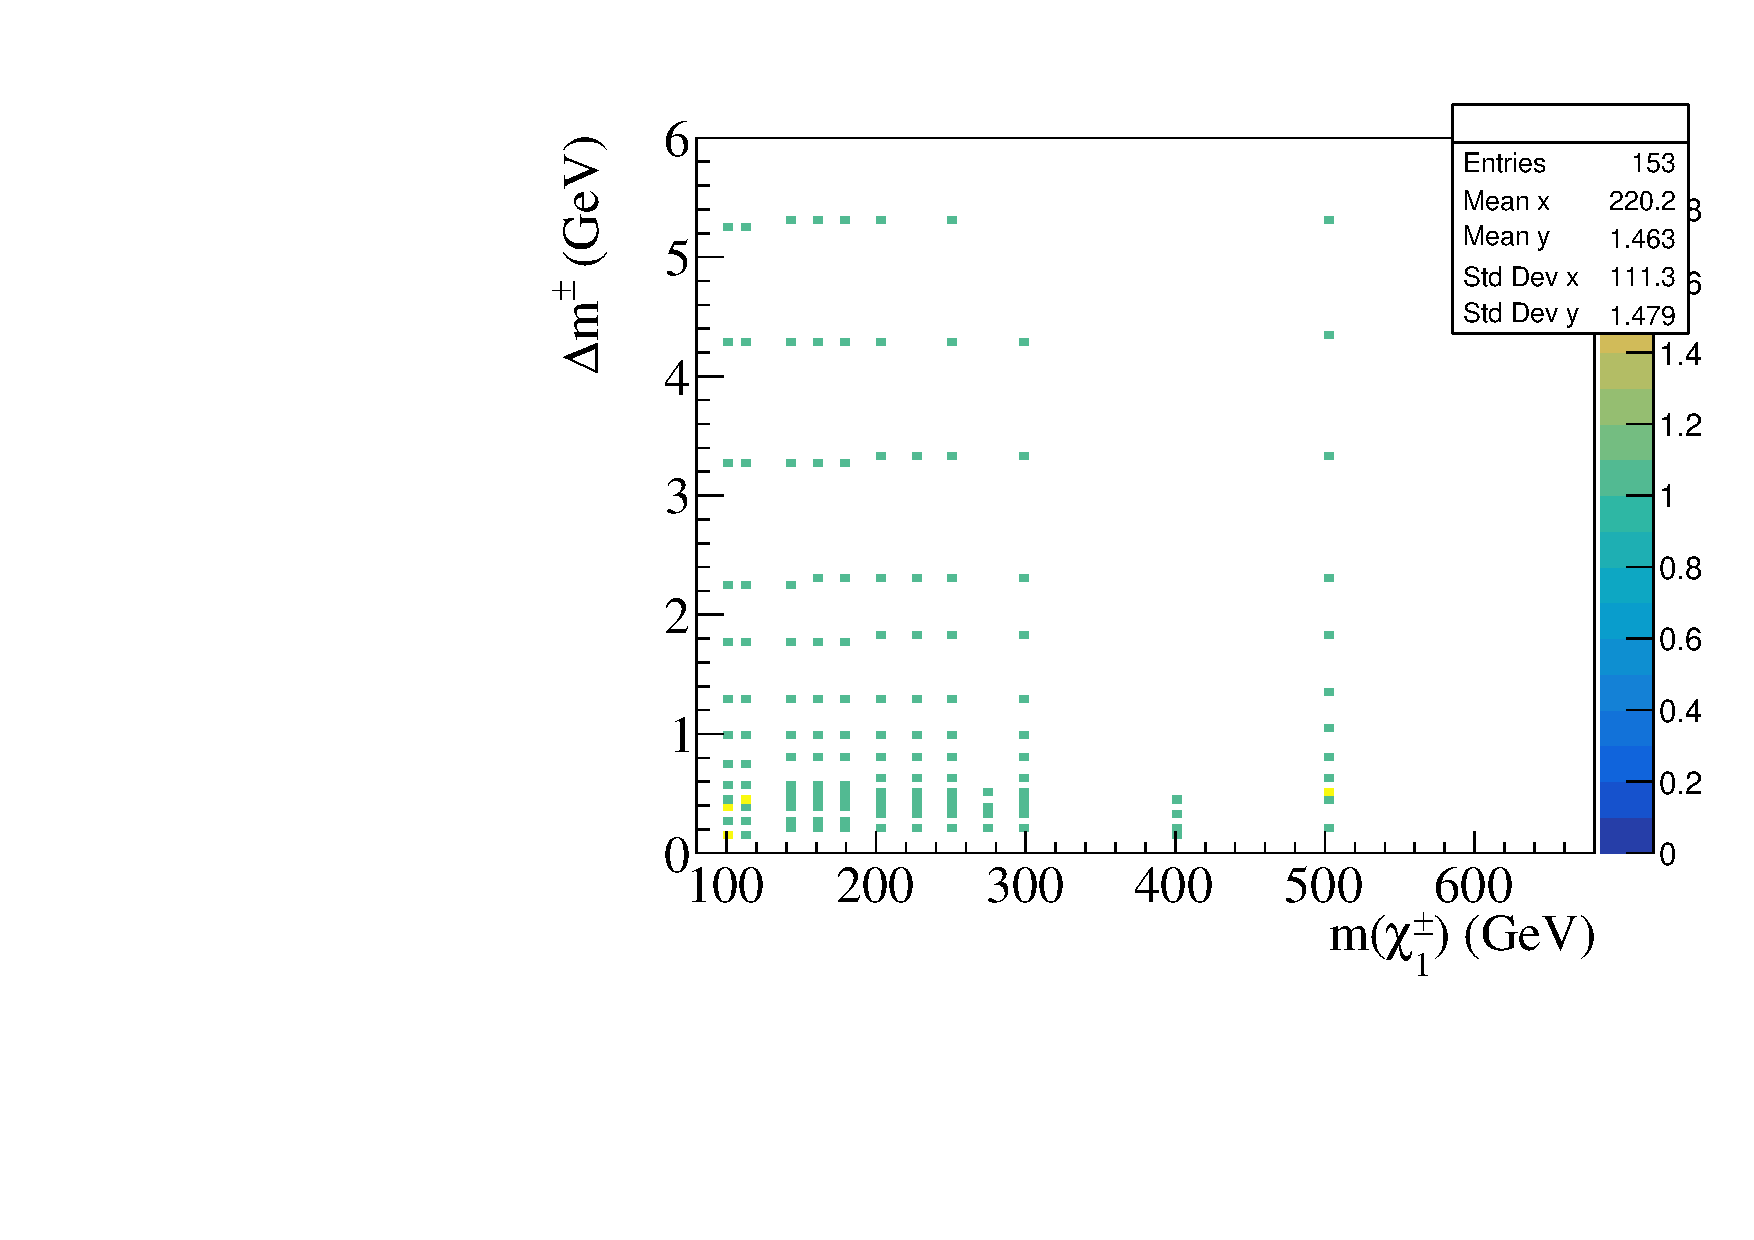
\includegraphics[width=0.80\linewidth]{plots/signal_scan/PureHiggsinoScan.pdf} \\
\caption[Distribution of the grid of model points chosen for simulation]{Distribution of the grid of model points chosen for simulation.}
\label{fig:signal-scan-grid}
\end{figure}

The lifetimes of the electroweakinos are determined from phase space using the spectrum generator package SUSYHIT \cite{Allanach:2001kg}. A scan is performed in the dimensions of $\Delta m^{\pm}$ and the higgsino mass.

The dominant decay of the chargino in such models is to hadrons, most often a single soft pion, via an off-shell W boson; we assume a branching fraction of 100\%. The Z$^{*}$ is assumed to decay primarily to hadrons, with a branching fraction to electrons and muons of 5\% each (10\% combined).



\subsection{Collected data samples}
\label{sec:data-samples}

We analyze the 13\TeV dataset collected during 2016, 2017, and 2018 with the CMS detector.
For 2016 and 2017 we used the \texttt{17Jul2018 re-reco} and \texttt{31Mar2018 re-reco} versions, respectively,
while for 2018 we used we used the \texttt{17Sep2018 re-reco} for periods A-C and a combination of the \texttt{22Jan2019 re-prompt reco} and the \texttt{prompt-reco} datasets for period D.
Table \ref{tab:DataSamples} lists the integrated luminosities for the primary datasets used,
split up by data-taking period, for each of the years.
The data set is measured to correspond to 137.2\fbinv using the BRIL Work Suite \cite{bril}.

\begin{table}[hp]
\centering
\caption{Data sets collected from three years of data-taking. All \lint are listed in \fbinv and are calculated using the BRIL Work Suite \cite{bril}.}
\label{tab:DataSamples}
{\footnotesize
\begin{tabular}{|lccccccccc|}
\hline
\textbf{2016 Data set} & \textbf{--} & B    & C    & D     & E    & F     & G    & H    & Total \\ \hline
MET                   & --          & 5.82 & 2.62 & 4.29  & 3.92 & 3.14 & 7.65 & 8.74 & 36.17 \\
SingleElectron        & --          & 5.81 & 2.62 & 4.29  & 4.06 & 3.13 & 7.64 & 8.73 & 36.27 \\
\textbf{2017 Data set} & --          & B    & C    & D     & E    & F     & G    & H    & Total \\ \hline
MET                   & --          & 4.57 & 8.91 & 2.42  & 10.36 & 15.13 &      & --   & 41.39 \\
SingleElectron        & --          & 4.70 & 9.26 & 4.43  & 10.02 & 13.03 &      & --   & 41.44 \\
\textbf{2018 Data set} & A           & B    & C    & D     & --   & --    & --   & --   & Total \\ \hline
MET                   & 14.01          & 5.06      & 6.72 & 32.65 & --   & --    & --   & --   & 58.43 \\ \hline
\end{tabular}
}
\end{table}





